\documentclass[10pt,fleqn]{article}
\newcommand{\name}[1]{\def\psettitlename{#1}}
\newcommand{\course}[1]{\def\psettitlecourse{#1}}
\newcommand{\rsection}[1]{\def\psettitlersection{#1}}
\newcommand{\psetnum}[1]{\def\psettitlepsetnum{#1}}
%\usepackage[journal=rsc]{chemstyle}
%\usepackage{mhchem}
\usepackage{amsmath}
\usepackage{amssymb}
\usepackage{amsfonts}
\usepackage{esint}
\usepackage{bbm}
\usepackage{amscd}
\usepackage{picinpar}
\usepackage[pdftex]{graphicx}
\usepackage{tikz}
\usepackage{indentfirst}
\usepackage{wrapfig}
\usepackage{units}
\usepackage{textcomp}
\usepackage[utf8x]{inputenc}
% \usepackage{feyn}
\usepackage{feynmp}
\usetikzlibrary{
  arrows,
  calc,
  decorations.pathmorphing,
  decorations.pathreplacing,
  decorations.markings,
  fadings,
  positioning,
  shapes
}

\DeclareGraphicsRule{*}{mps}{*}{}
\newcommand{\ud}{\mathrm{d}}
\newcommand{\ue}{\mathrm{e}}
\newcommand{\ui}{\mathrm{i}}
\newcommand{\res}{\mathrm{Res}}
\newcommand{\Tr}{\mathrm{Tr}}
\newcommand{\dsum}{\displaystyle\sum}
\newcommand{\dprod}{\displaystyle\prod}
\newcommand{\dlim}{\displaystyle\lim}
\newcommand{\dint}{\displaystyle\int}
\newcommand{\fsno}[1]{{\!\not\!{#1}}}
\newcommand{\eqar}[1]
{
  \begin{align*}
    #1
  \end{align*}
}
\newcommand{\texp}[2]{\ensuremath{{#1}\times10^{#2}}}
\newcommand{\dexp}[2]{\ensuremath{{#1}\cdot10^{#2}}}
\newcommand{\eval}[2]{{\left.{#1}\right|_{#2}}}
\newcommand{\paren}[1]{{\left({#1}\right)}}
\newcommand{\lparen}[1]{{\left({#1}\right.}}
\newcommand{\rparen}[1]{{\left.{#1}\right)}}
\newcommand{\abs}[1]{{\left|{#1}\right|}}
\newcommand{\sqr}[1]{{\left[{#1}\right]}}
\newcommand{\crly}[1]{{\left\{{#1}\right\}}}
\newcommand{\angl}[1]{{\left\langle{#1}\right\rangle}}
\newcommand{\tpdiff}[4][{}]{{\paren{\frac{\partial^{#1} {#2}}{\partial {#3}{}^{#1}}}_{#4}}}
\newcommand{\tpsdiff}[4][{}]{{\paren{\frac{\partial^{#1}}{\partial {#3}{}^{#1}}{#2}}_{#4}}}
\newcommand{\pdiff}[3][{}]{{\frac{\partial^{#1} {#2}}{\partial {#3}{}^{#1}}}}
\newcommand{\diff}[3][{}]{{\frac{\ud^{#1} {#2}}{\ud {#3}{}^{#1}}}}
\newcommand{\psdiff}[3][{}]{{\frac{\partial^{#1}}{\partial {#3}{}^{#1}} {#2}}}
\newcommand{\sdiff}[3][{}]{{\frac{\ud^{#1}}{\ud {#3}{}^{#1}} {#2}}}
\newcommand{\tpddiff}[4][{}]{{\left(\dfrac{\partial^{#1} {#2}}{\partial {#3}{}^{#1}}\right)_{#4}}}
\newcommand{\tpsddiff}[4][{}]{{\paren{\dfrac{\partial^{#1}}{\partial {#3}{}^{#1}}{#2}}_{#4}}}
\newcommand{\pddiff}[3][{}]{{\dfrac{\partial^{#1} {#2}}{\partial {#3}{}^{#1}}}}
\newcommand{\ddiff}[3][{}]{{\dfrac{\ud^{#1} {#2}}{\ud {#3}{}^{#1}}}}
\newcommand{\psddiff}[3][{}]{{\frac{\partial^{#1}}{\partial{}^{#1} {#3}} {#2}}}
\newcommand{\sddiff}[3][{}]{{\frac{\ud^{#1}}{\ud {#3}{}^{#1}} {#2}}}
\usepackage{fancyhdr}
\usepackage{multirow}
\usepackage{fontenc}
%\usepackage{tipa}
\usepackage{ulem}
\usepackage{color}
\usepackage{cancel}
\newcommand{\hcancel}[2][black]{\setbox0=\hbox{#2}%
\rlap{\raisebox{.45\ht0}{\textcolor{#1}{\rule{\wd0}{1pt}}}}#2}
\pagestyle{fancy}
\setlength{\headheight}{67pt}
\fancyhead{}
\fancyfoot{}
\fancyfoot[C]{\thepage}
\fancyhead[R]
{
\psettitlename \\
\psettitlecourse{} Problem Set \psettitlepsetnum \\
\ifx\psettitlersection\empty
\else
Recitation Section \psettitlersection
\fi
}
\renewcommand{\footruleskip}{0pt}
\renewcommand{\headrulewidth}{0.4pt}
\renewcommand{\footrulewidth}{0pt}
\addtolength{\hoffset}{-1.3cm}
\addtolength{\voffset}{-2cm}
\addtolength{\textwidth}{3cm}
\addtolength{\textheight}{2.5cm}
\renewcommand{\footskip}{10pt}
\setlength{\headwidth}{\textwidth}
\setlength{\headsep}{20pt}
\setlength{\marginparwidth}{0pt}
\parindent=0pt
\psetnum{1}
\course{8.422}
\rsection{1}
\name{Yichao Yu}
\renewcommand{\thesection}{\arabic{section}.}
\renewcommand{\thesubsection}{(\alph{subsection})}
\renewcommand{\thesubsubsection}{\roman{subsubsection}.}

\begin{document}
\section{}
\subsection{}
\eqar{
  \angl{\alpha|\beta}=&\exp\paren{-\frac{\abs{\alpha}^2+\abs{\beta}^2}2}
  \sum_{n}\frac{(\alpha^*)^n\beta^n}{n!}\\
  =&\exp\paren{-\frac{\abs{\alpha}^2+\abs{\beta}^2}2+\alpha^*\beta}
}
\subsection{}
\eqar{
  \langle n\int |\alpha\rangle\langle\alpha|\frac{\ud^2\alpha}{\pi}|m\rangle=&\ue^{-\abs{\alpha}^2}\int \frac{\abs{\alpha}^{2n}\alpha^{m-n}}{\sqrt{n!m!}}\abs{\alpha}\frac{\ud\abs{\alpha}\ud\theta}{\pi}\\
  =&\delta_{mn}\ue^{-\abs{\alpha}^2}\int \frac{\abs{\alpha}^{2n}}{n!}\ud\abs{\alpha}^2\\
  =&\delta_{mn}
}
\subsection{}
\eqar{
  D\paren{\alpha}|0\rangle=&\exp\paren{\alpha a^\dagger-\alpha^*a}|0\rangle\\
  =&\ue^{\alpha a^\dagger}\ue^{-\alpha^*a}\ue^{\alpha\alpha^*\sqr{a^\dagger, a} / 2}|0\rangle\\
  =&\exp\paren{-\frac{\abs{\alpha}^2}2}\ue^{\alpha a^\dagger}|0\rangle\\
  =&|\alpha\rangle
}
\subsection{}
\eqar{
  \angl{E_x}=&E_0\sin\paren{kz}\angl{a + a^\dagger}\\
  =&E_0\sin\paren{kz}\paren{\alpha + \alpha^*}\\
  \angl{E_x^2}=&E_0^2\sin^2\paren{kz}\angl{\paren{a + a^\dagger}^2}\\
  =&E_0^2\sin^2\paren{kz}\angl{a^2 + 1 + 2a^\dagger a+{a^\dagger}^2}\\
  =&E_0^2\sin^2\paren{kz}\paren{\paren{\alpha + \alpha^*}^2 + 1}\\
  \sqrt{\angl{\Delta E_x^2}}=&E_0\sin\paren{kz}
}
The deviation of the field does not change (even for vacuum) because the coherent state is just a displacement of the vacuum state.

\subsection{}
For number state
\eqar{
  P\paren{\phi}=&\frac1{2\pi}
}
so the number state has equal probability of having any phase.
\eqar{
  P\paren{\phi, \theta}=&\frac1{2\pi}\abs{\sum_n\angl{n|\ue^{-\ui n\phi}|\paren{\abs{\alpha}\ue^{\ui\theta}}}}^2\\
  =&\frac1{2\pi}\abs{\sum_n\ue^{-\ui n\paren{\phi-\theta}}\angl{n|\paren{\abs{\alpha}}}}^2\\
  =&P\paren{\phi-\theta, 0}
  \intertext{Therefore $P$ rotates in the same way as the phase of $\alpha$ changes}
  P\paren{\phi, 0}=&\frac1{2\pi}\abs{\sum_n\angl{n|\ue^{-\ui n\phi}|\paren{\abs{\alpha}}}}^2\\
  =&\frac{\ue^{-\abs{\alpha}^2}}{2\pi}\abs{\sum_n\ue^{-\ui n\phi}\frac{\abs{\alpha}^n}{\sqrt{n!}}}^2
}
So $P\paren{\phi, 0}$ is symmetrically distributed and maximized at $\phi=0$ (therefore $P\paren{\phi, \theta}$ is maximized when $\phi=\theta$) if $\abs{\alpha}\neq0$. Therefore the expected value of $\phi$ (when $\alpha\neq0$) is $\theta$.

\section{}
\subsection{}
\eqar{
  \frac{V_\psi}{V_0}=&\frac14\langle\psi,0|\paren{a^\dagger+b^\dagger}\paren{a+b}\paren{a^\dagger-b^\dagger}\paren{a-b}|\psi,0\rangle\\
  =&\frac14\langle\psi,0|a^\dagger\paren{aa^\dagger-ab^\dagger+ba^\dagger-bb^\dagger}a|\psi,0\rangle\\
  =&\frac14\langle a^\dagger a^\dagger aa\rangle
}
\subsection{}
\eqar{
  g_{cl}^{(2)}\paren{0}=&\frac{\angl{I^2}}{\angl{I}^2}\\
  =&1+\frac{\angl{I^2}-\angl{I}^2}{\angl{I}^2}\\
  =&1+\frac{\angl{\paren{I-\angl{I}}^2}}{\angl{I}^2}\\
  \geqslant&1
}
\subsection{}
\eqar{
  g^{(2)}_{\alpha}=&\frac{\abs{a}^4}{\abs{a}^4}\\
  =&1\\
  g^{(2)}_{n=2}=&\frac{2\cdot 3}{2^2}\\
  =&\frac32
}
\subsection{}
\eqar{
  \langle\psi_3|\psi_3\rangle=&\paren{1+\ue^{2\abs{\alpha}^2}}\\
  \langle\psi_4|\psi_4\rangle=&\paren{1-\ue^{2\abs{\alpha}^2}}\\
  g^{(2)}_{3,4}=&\frac{\langle\psi_{3,4}|a^\dagger a^\dagger a a|\psi_{3,4}\rangle\langle\psi_{3,4}|\psi_{3,4}\rangle}{\langle\psi_{3,4}|a^\dagger a|\psi_{3,4}\rangle^2}\\
  =&\frac{\paren{\langle\alpha|\pm\langle-\alpha|}a^\dagger a^\dagger a a\paren{|\alpha\rangle\pm|-\alpha\rangle}\paren{1\pm\ue^{2\abs{\alpha}^2}}}{\paren{\langle\alpha|\pm\langle-\alpha|}a^\dagger a\paren{|\alpha\rangle\pm|-\alpha\rangle}^2}\\
  =&\frac{\abs{\alpha}^4\paren{\langle\alpha|\pm\langle-\alpha|}\paren{|\alpha\rangle\pm|-\alpha\rangle}\paren{1\pm\ue^{2\abs{\alpha}^2}}}{\abs{\alpha}^4\paren{\langle\alpha|\mp\langle-\alpha|}\paren{|\alpha\rangle\mp|-\alpha\rangle}^2}\\
  =&\paren{\frac{1\pm\ue^{2\abs{\alpha}^2}}{1\mp\ue^{2\abs{\alpha}^2}}}^2
}
Therefore $g^{(2)}$ can be smaller than $1$ for $\psi_4$.

\section{}
\subsection{}
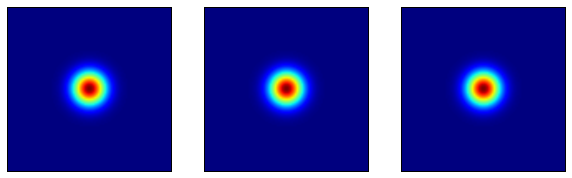
\includegraphics[width=15cm]{3-1-0_4.png}\\
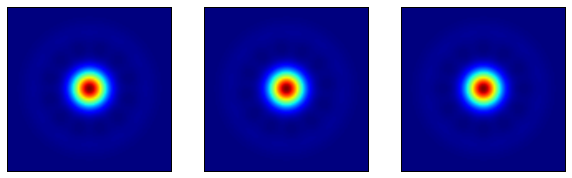
\includegraphics[width=15cm]{3-1-1_4.png}\\
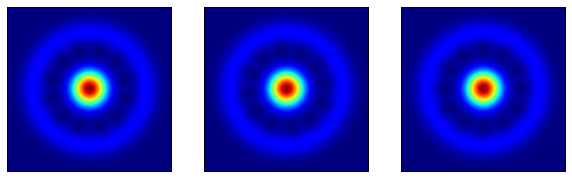
\includegraphics[width=15cm]{3-1-2_4.png}\\
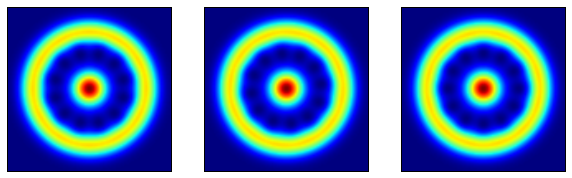
\includegraphics[width=15cm]{3-1-3_4.png}\\
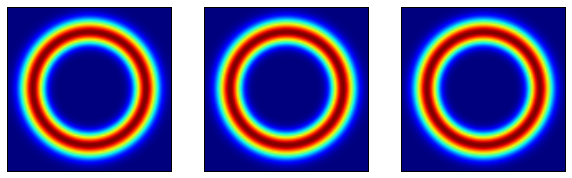
\includegraphics[width=15cm]{3-1-4_4.png}\\
These are not minimum uncertainty states (except when it's $|0\rangle$) and not squeezed states.

\subsection{}
$\alpha=3\ui$
Linear scale\\
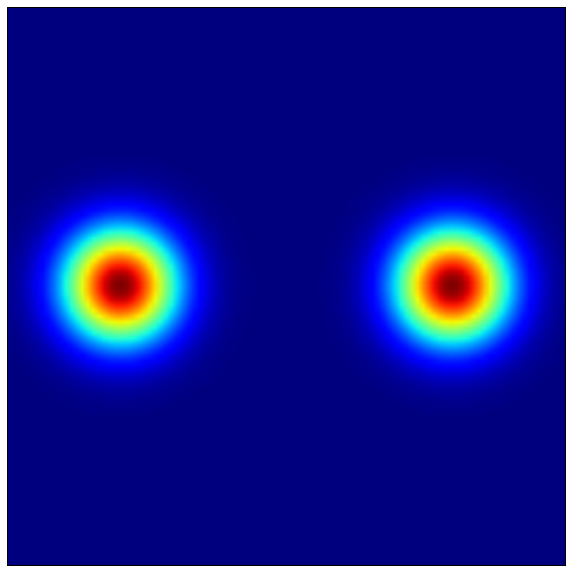
\includegraphics[width=10cm]{3-2-lin.png}\\
Log scale\\
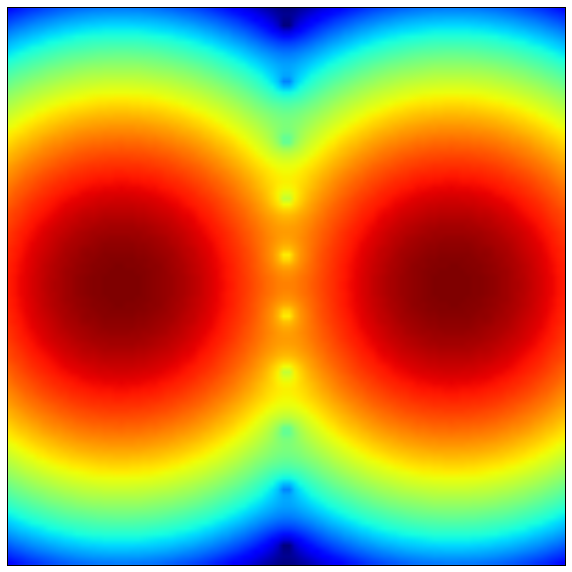
\includegraphics[width=10cm]{3-2-log.png}\\
Interference fringes appears because the two wavefunction overlaps.

\subsection{}
States with $\phi=0, \dfrac\pi4, \dfrac\pi2$ and $N=5,10,15,20,15$\\
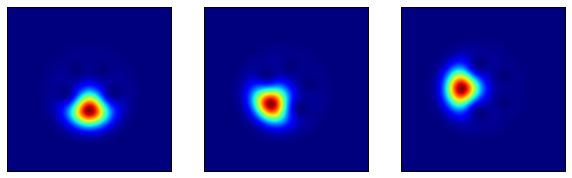
\includegraphics[width=15cm]{3-3-5.png}\\
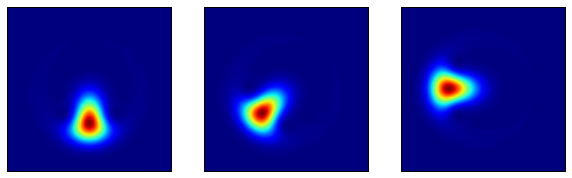
\includegraphics[width=15cm]{3-3-10.png}\\
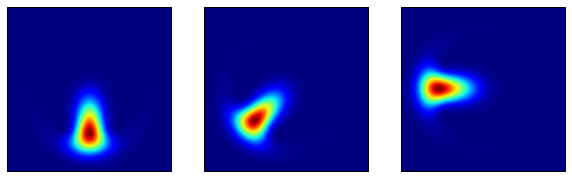
\includegraphics[width=15cm]{3-3-15.png}\\
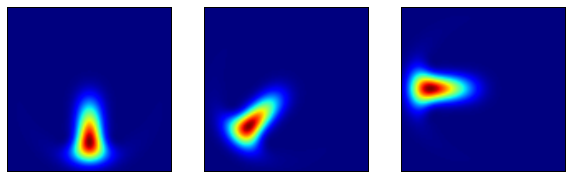
\includegraphics[width=15cm]{3-3-20.png}\\
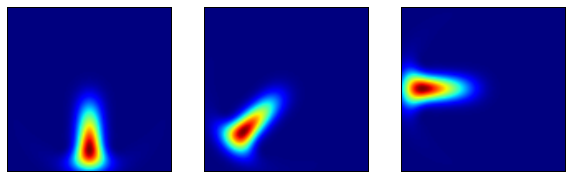
\includegraphics[width=15cm]{3-3-25.png}\\
With $N=2000$ and compare to $N=1$\\
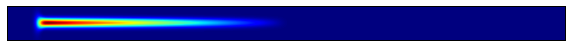
\includegraphics[width=15cm]{3-3-2000.png}\\
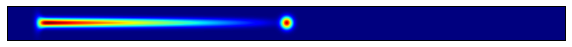
\includegraphics[width=15cm]{3-3-2000_0.png}\\
These are not squeezed states since they do not decrease the uncertainty in one direction.

\subsection{}
(Transposed and not at the same scale)\\
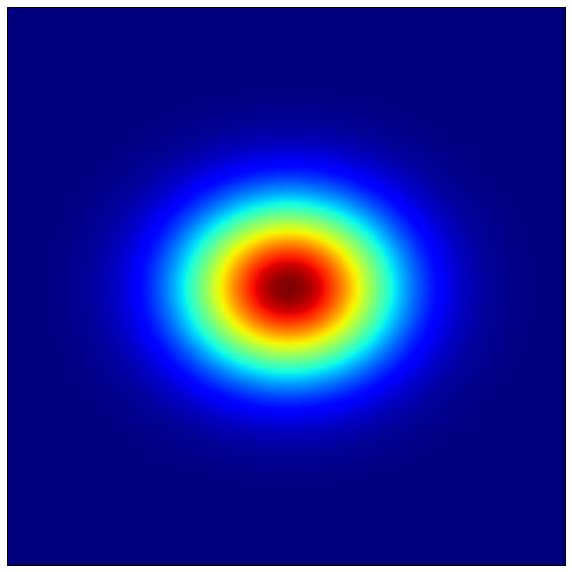
\includegraphics[width=15cm]{3-4-02.png}\\
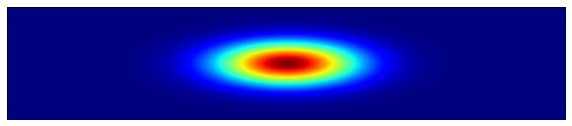
\includegraphics[width=15cm]{3-4-12.png}\\

\includegraphics[width=15cm]{3-4-4.png}

\subsection{}
$\xi t$ from $0$ to $\dfrac{25}{24}$ every $\dfrac1{120}$\\
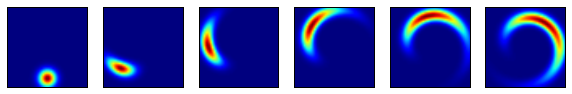
\includegraphics[width=15cm]{3-5-0.png}\\
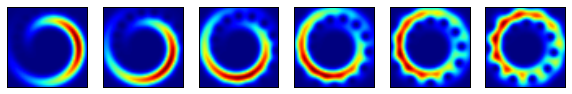
\includegraphics[width=15cm]{3-5-1.png}\\
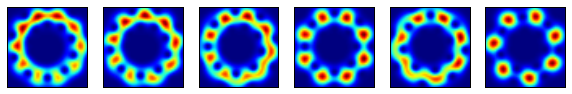
\includegraphics[width=15cm]{3-5-2.png}\\
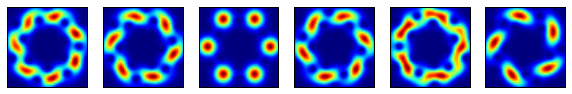
\includegraphics[width=15cm]{3-5-3.png}\\
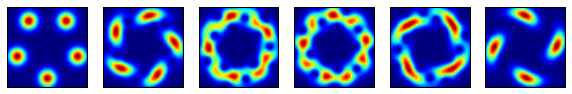
\includegraphics[width=15cm]{3-5-4.png}\\
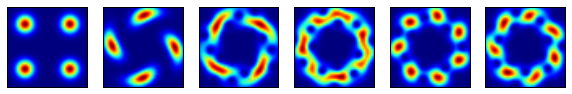
\includegraphics[width=15cm]{3-5-5.png}\\
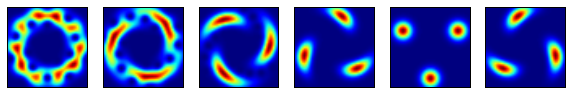
\includegraphics[width=15cm]{3-5-6.png}\\
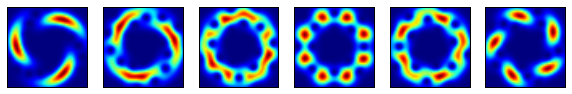
\includegraphics[width=15cm]{3-5-7.png}\\
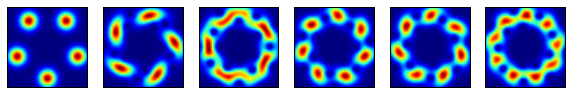
\includegraphics[width=15cm]{3-5-8.png}\\
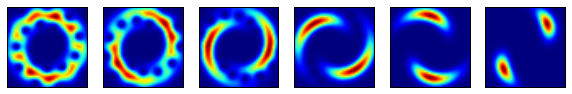
\includegraphics[width=15cm]{3-5-9.png}\\
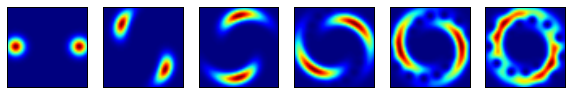
\includegraphics[width=15cm]{3-5-10.png}\\
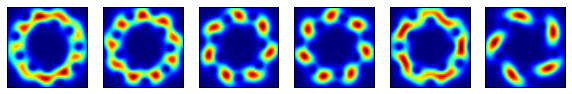
\includegraphics[width=15cm]{3-5-11.png}\\
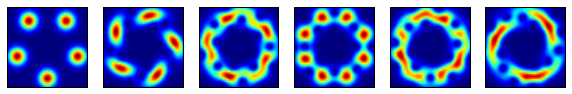
\includegraphics[width=15cm]{3-5-12.png}\\
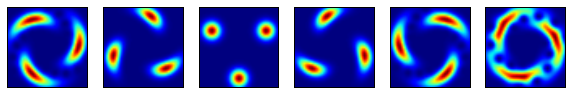
\includegraphics[width=15cm]{3-5-13.png}\\
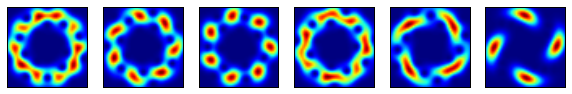
\includegraphics[width=15cm]{3-5-14.png}\\
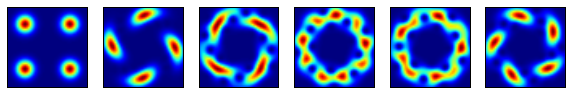
\includegraphics[width=15cm]{3-5-15.png}\\
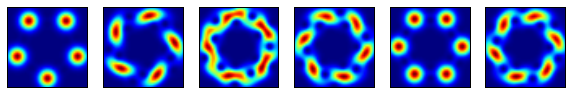
\includegraphics[width=15cm]{3-5-16.png}\\
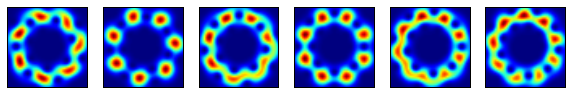
\includegraphics[width=15cm]{3-5-17.png}\\
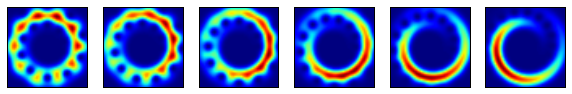
\includegraphics[width=15cm]{3-5-18.png}\\
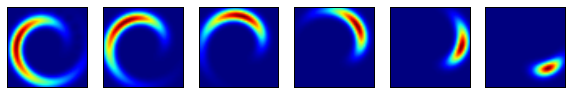
\includegraphics[width=15cm]{3-5-19.png}\\
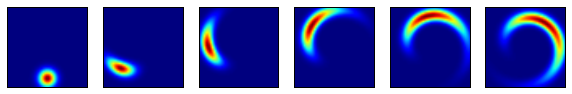
\includegraphics[width=15cm]{3-5-20.png}\\
It become two superposed coherent state when $\xi t=\dfrac12$ and come back to its original state when $\xi t=1$. For a video of the evolution, see ``http://git.yuyichao.com/yuyichao/8-422/raw/master/pset/pset1/3-5.webm''.

\end{document}
